This chapter describes all the steps that were taken in the design of a controller for the master motor of the rolling mill plant. Along the way all the design choices will be explained and substantiated.

\section{Master motor}
The master motor is the one that pulls the strip and winds it up on a spool. The left motor was chosen as master since its RPM at working current is higher than the right motor.  This is necessary since when the strip is compressed to reduce its thickness it extends. The speed of the winding motor needs to be higher than the feeding motor. Figure \ref{fig:LM_RPM_curr} shows a plot of the motor characteristics and table \ref{tab:LM_operating_region} shows the currents for different operating points.

\begin{figure}[htbp]
\centering
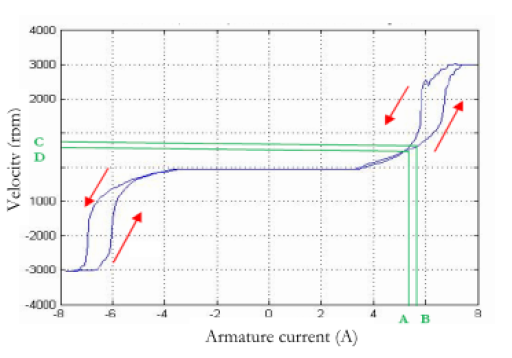
\includegraphics[width = .7\textwidth]{pics/LM_RPM_Current.png}
\caption{Rotational Velocity of the Left motor in function of the Current}
\label{fig:LM_RPM_curr}
\end{figure}

\begin{table}[H]
	\centering
		\begin{tabular}{c|c}
        \toprule
			Armature current [A] & Angular velocity [RPM] \\ \midrule
            5.4 & 530.7 \\
            5.7 & 649.8 \\
		\end{tabular}
	\caption{Operating points of the left motor}
	\label{tab:LM_operating_region}
\end{table}

\FloatBarrier
\section{Identifying the transfer function}

The transfer function of the left motor was identified using matlab. To do this, velocity was sampled for a step input. Since the motor works around a given operating region, it was started from the lower setpoint current and an the step increased the current to the higher setpoint. The transient from stopped to the operating is not very interesting. The behaviour of the change in velocity was used to calculate a transfer function using the least squares method. 

Figure \ref{fig:LM_id} shows the sampled data points and the curve that corresponds to the transfer function of the left motor (equation \ref{eq:LM_TF}).

\begin{align}
	G(s) = \frac{5.398}{3.642S+1}
    \label{eq:LM_TF}
\end{align}

\begin{figure}[htbp]
\centering
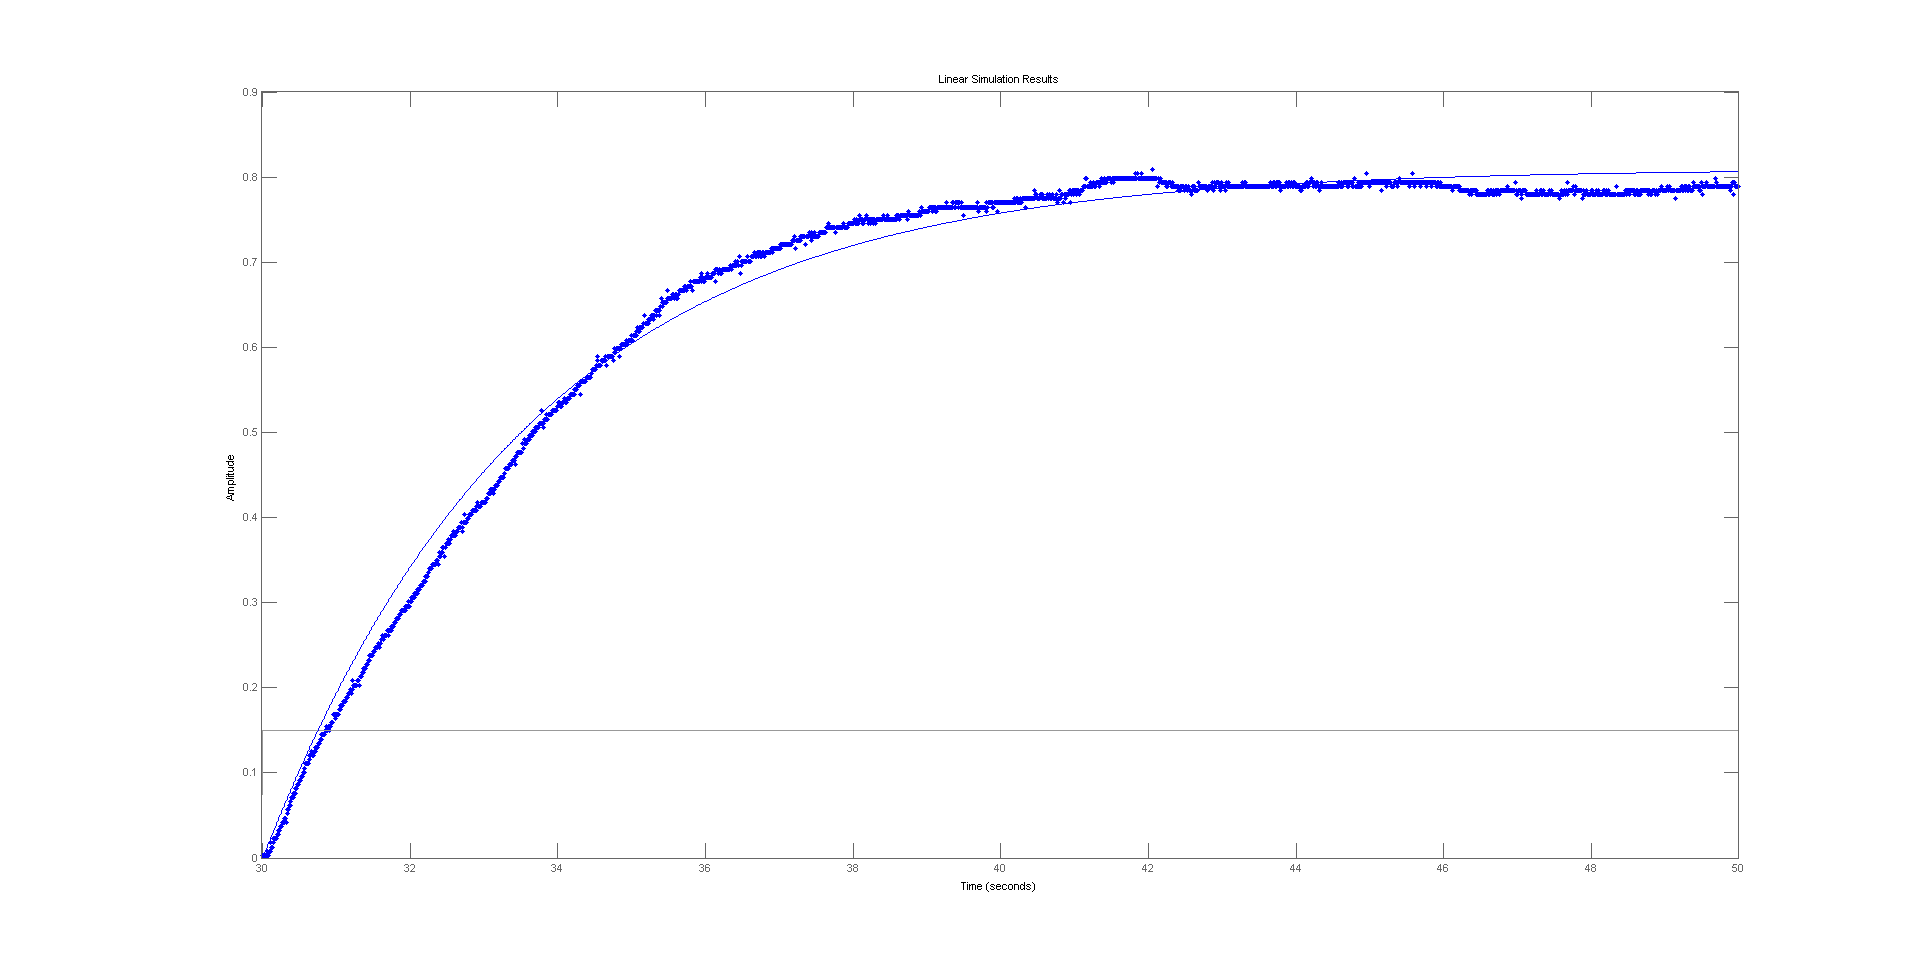
\includegraphics[width = \textwidth]{identification_step_setpoints.png}
\caption{Sampled data with the fitted curve from the calculated transfer function}
\label{fig:LM_id}
\end{figure}

\FloatBarrier
\section{Controller design}
This controller needs to be able to keep the master velocity stable and constant. A PI controller has been chosen to control this motor. 

To design this PI controller the root locus method has been used. The zero of the PI controller was used to cancel the pole of the transfer function of the left motor. This was done as follows:

The transfer function for the left motor was transformed to make the pole location visible.
\begin{align}
	G(s) &= \frac{5.398}{3.642S+1} \\[12pt]
    &= \frac{1.482}{s+0.274} \nonumber
\end{align}

The same was done for the PI controller so that the zero location becomes easily visible.
\begin{align}
    C(s) &= K_p + \frac{K_i}{s}\\[12pt]
    &= K_p \left(\frac{s+\frac{K_i}{K_p}}{s} \right) \nonumber
\end{align}

To use the zero to compensate the pole of the left motor the nominator of the controller $C(s)$ needs to be the same of the denominator of the left motor $G(s)$. This means that $\frac{K_i}{K_p} = 0.294$

Using these previous equations $K_p$ can be chosen using the root locus tool from matlab. The total system, without $K_p$ equates to:

\begin{align}
    Sys(s) &= \frac{1.482}{s+0.274} \cdot \frac{s+0.274}{s} \\[12pt]
     &= \frac{1.482}{s}
\end{align}

Entering this system in the matlab root locus tool provides us with the  root locus plot seen on figure \ref{fig:LM_rl}. The gain can be chosen arbitrarily, but larger than 0.

\begin{figure}[htbp]
\centering
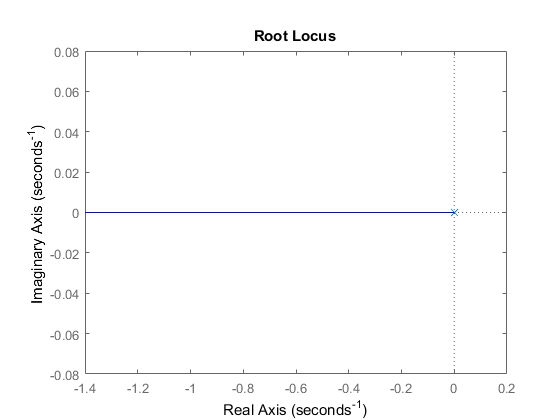
\includegraphics[width = .7\textwidth]{pics/LM_cont_rlocus.png}
\caption{Root locus plot for the left motor with a PI controller}
\label{fig:LM_rl}
\end{figure}

Several different values were used in simulation in simulink (figure \ref{fig:LM_SIM_KP050}, figure \ref{fig:LM_SIM_KP144} and figure \ref{fig:LM_SIM_KP200})


\begin{figure}[htbp]
\centering
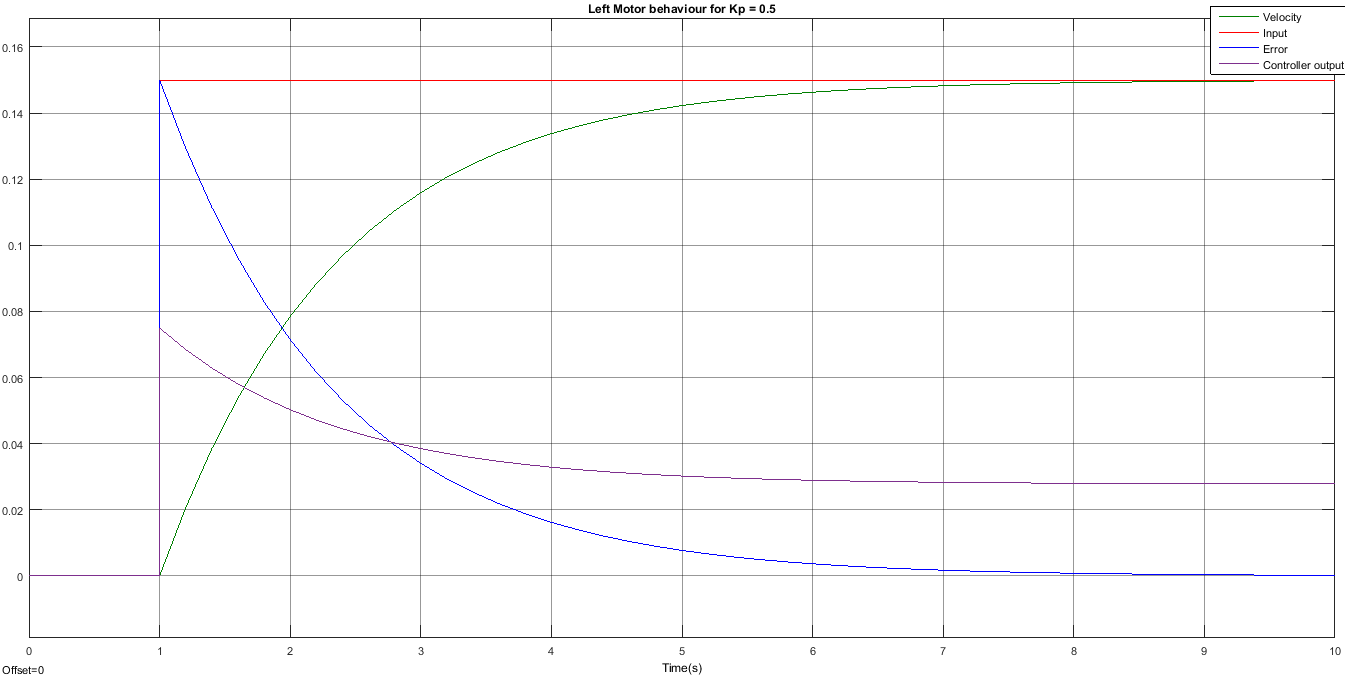
\includegraphics[width = \textwidth]{pics/LM_KP050_Sim.png}
\caption{Simulink simulation of the left motor behaviour for $K_p = 0.5$}
\label{fig:LM_SIM_KP050}
\end{figure}

\begin{figure}[htbp]
\centering
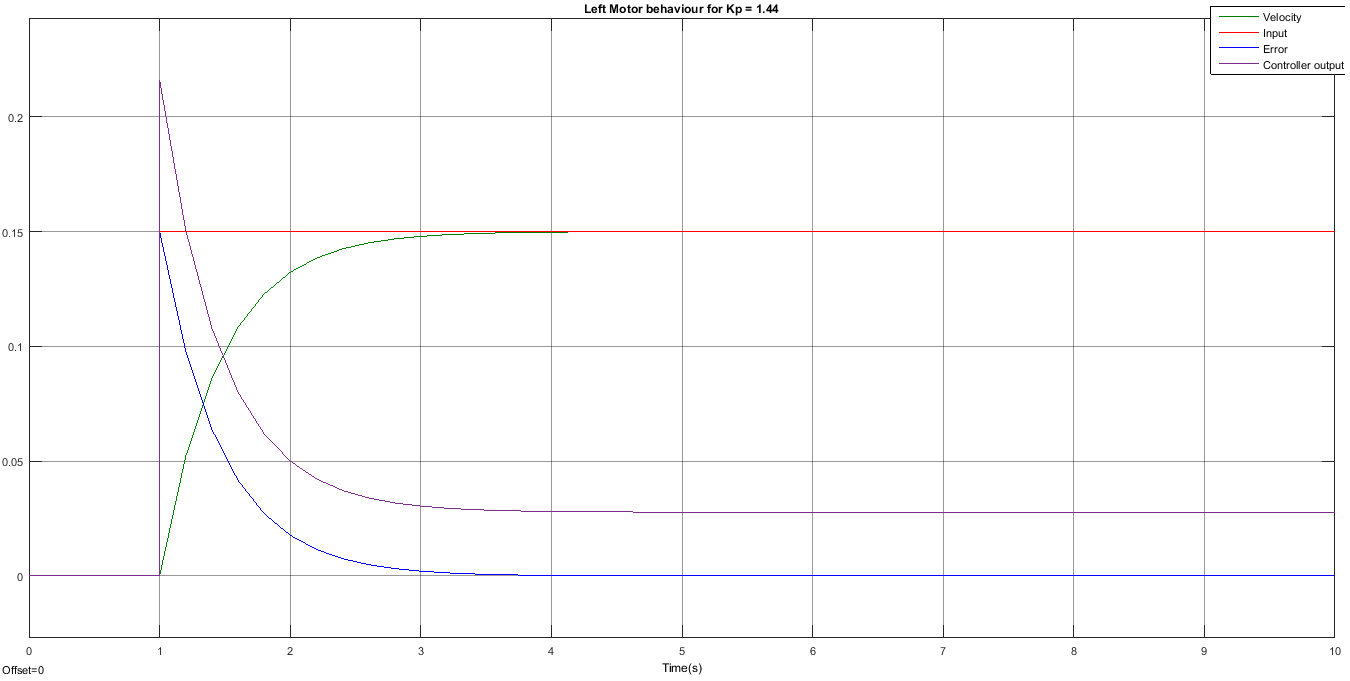
\includegraphics[width = \textwidth]{pics/LM_KP144_Sim.png}
\caption{Simulink simulation of the left motor behaviour for $K_p = 1.44$}
\label{fig:LM_SIM_KP144}
\end{figure}

\begin{figure}[htbp]
\centering
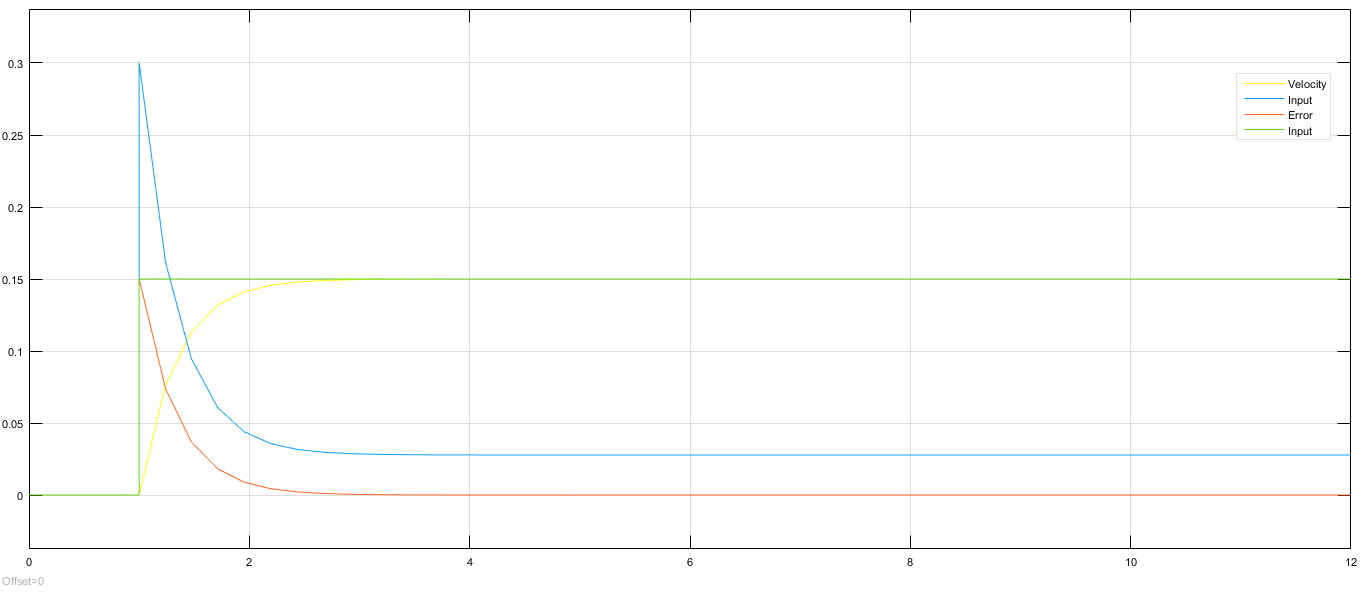
\includegraphics[width = \textwidth]{pics/LM_KP200_sim.png}
\caption{Simulink simulation of the left motor behaviour for $K_p = 2$}
\label{fig:LM_SIM_KP200}
\end{figure}

\FloatBarrier

Using the previous equations and calculated values, a discrete time PI controller could be implemented in matlab using the DAQ system.

The controller was tested in practice for different values of the $K_p$ (see figure \ref{fig:LM_KP050}, figure \ref{fig:LM_KP144} and figure \ref{fig:LM_KP200}). Based on these measurements $K_p = 1.44$ was chosen. $K_p = 0.5$ has a quite long settling time with a larger overshoot than $K_p = 1.44$.  Since $\frac{K_i}{K_p} = 0.294$, $K_i = 0.3954$. In none of the simulations is there overshoot present while all of the practical experiments do. This is because the transfer function of the motor was reduced to a first order system while in practice it behaves as a non linear system of higher order. 

\begin{figure}[htbp]
\centering
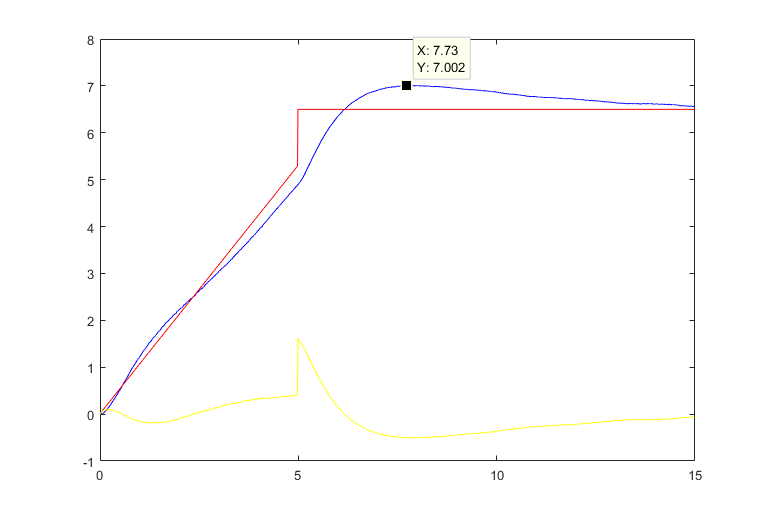
\includegraphics[width = .7\textwidth]{pics/LM_KP050a.png}
\caption{Response of the left motor behaviour for $K_p = 0.5$ to the red curve as input.}
\label{fig:LM_KP050}
\end{figure}

\begin{figure}[htbp]
\centering
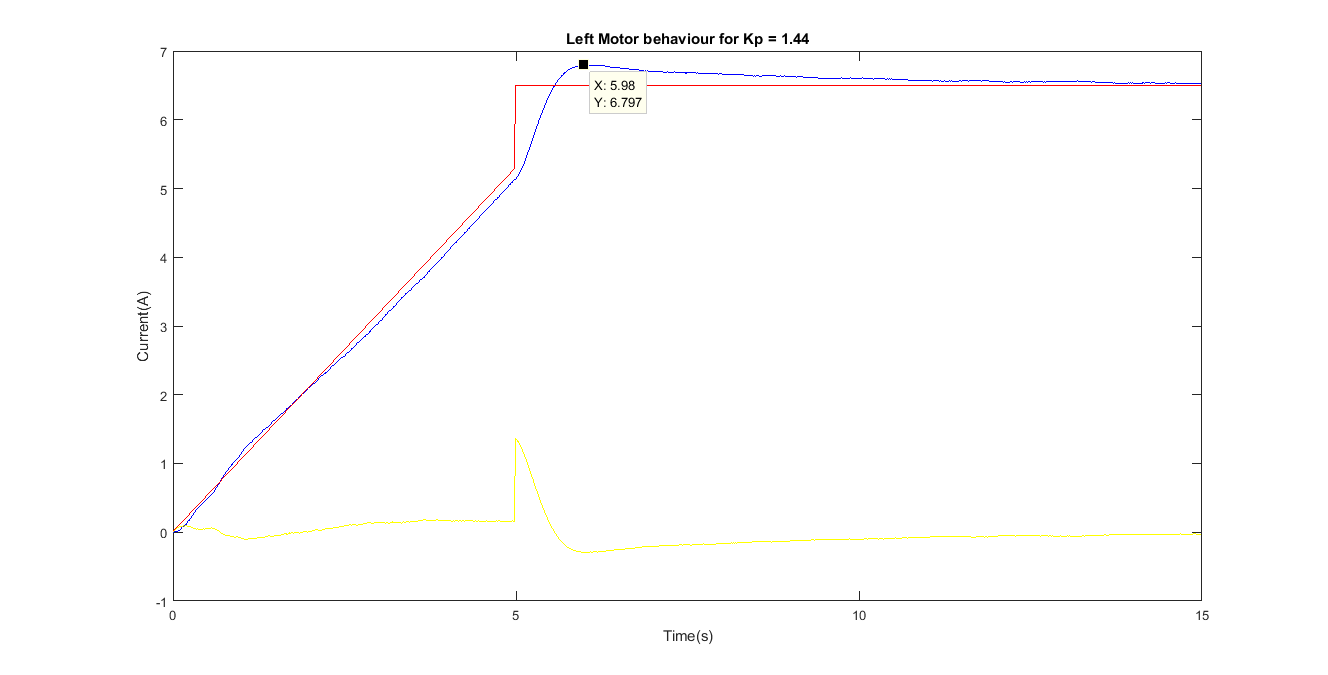
\includegraphics[width = .7\textwidth]{pics/LM_KP144.png}
\caption{Response of the left motor behaviour for $K_p = 1.44$ to the red curve as input.}
\label{fig:LM_KP144}
\end{figure}

\begin{figure}[htbp]
\centering
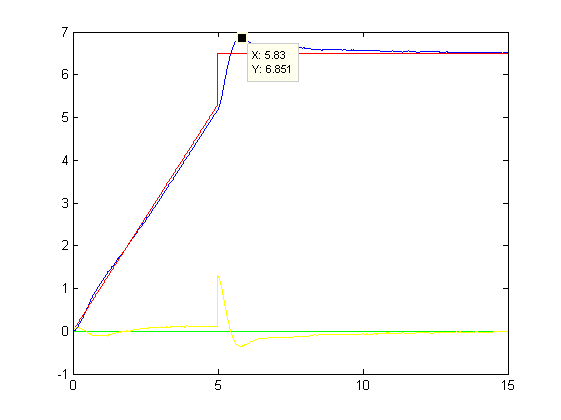
\includegraphics[width = .7\textwidth]{pics/LM_KP200.png}
\caption{Response of the left motor behaviour for $K_p = 2$ to the red curve as input.}
\label{fig:LM_KP200}
\end{figure}

\section{Conclusions}
For the controller of the whole plant cascade control was chosen with a grey box approach. The left motor was designated as the master motor. So first this motor was identified using the step response around the operating point. 

After the system had been identified a controller could be devised to control the velocity of the motor. A PI controller was chosen to keep the velocity stable and to reject disturbances. The PI controller was designed to cancel the pole of the transfer function of the motor. Multiple values of the feedback gain were simulated and tested in practice. Finally $K_p = 1.44$ was chosen to be used in the final plant controller.

